%LTeX: language=es
\documentclass[aspectratio=169]{beamer}
\usetheme{Boadilla}
\usecolortheme{whale}
\usepackage[utf8]{inputenc}
\usepackage[spanish,es-nodecimaldot]{babel}
\usepackage{amsmath}
\usepackage{amsfonts}
\usepackage{amssymb}
\usepackage{graphicx}
\graphicspath{{./figures/}}
\usepackage{ragged2e}
\usepackage{xcolor}
% \usepackage[outputdir={D:/tmp}]{minted}
\usepackage[outputdir={/home/espinosa/tmp}]{minted}
\usepackage{caption}
\setminted[latex]{xleftmargin=1cm}
\setbeamercolor{bibliography entry title}{fg=blue!50!cyan}
\setbeamercolor{bibliography entry author}{fg=violet}
\setbeamercolor{bibliography entry location}{fg=green}
\setbeamercolor{bibliography entry note}{fg=orange}
\setbeamerfont{bibliography entry title}{size=\footnotesize,series=\bfseries}
\setbeamerfont{bibliography entry author}{size=\small}
\setbeamerfont{bibliography entry location}{size=\small}
\setbeamerfont{bibliography entry note}{size=\tiny}
\usepackage{hyperref}
\hypersetup{
  colorlinks=true,
  linkcolor=cyan,
  filecolor=magenta,
  urlcolor=cyan,
}
\setbeamertemplate{navigation symbols}{}
\setbeamertemplate{caption}[numbered]
\definecolor{LightGray}{gray}{0.9}
\definecolor{darkgreen}{rgb}{0,0.6,0}
\definecolor{codegray}{rgb}{0.5,0.5,0.5}
\renewcommand{\listingscaption}{Código}
\setminted{
    frame=lines,
    framesep=2mm,
    baselinestretch=1.2,
    bgcolor=LightGray,
    fontsize=\footnotesize,
    linenos,
    autogobble
}
\DeclareCaptionFormat{mListing}{%
\hrule%
\textbf{#1}#2#3%
\hrule
}
\captionsetup[listing]{
  justification=raggedright,
  singlelinecheck=off,
  labelfont=bf,
  labelsep=space,
  format=mListing,
}
\title{Introducción a \LaTeX}
\subtitle{Usando paquetes}
\author[Carlos Espinosa]{Dr. Carlos Crispín Espinosa Ponce}
\institute[FC-UNAM]{Facultad de Ciencias\\Universidad Nacional Autónoma de México}

\begin{document}
  \begin{frame}
    \maketitle
  \end{frame}
  \section{Introducción}
    \begin{frame}
      \frametitle{¿Qué son los paquetes de \LaTeX?}
        \justifying
        \onslide<1,2,3>{
          Como hemos visto, \LaTeX\ es un \emph{markup language} que permite la escritura de documentos de alta calidad. Su principal diferencia con los procesadores de texto convencionales es el manejo del contenido y el formato de manera independiente.

        }
        \onslide<2,3>{
          Una de las diferencias que existen entre trabajar con \LaTeX\ y, por ejemplo, Word es las herramientas disponibles. En los procesadores de texto convencionales se cargan todas las herramientas que se tienen cuando se abre el programa.\footnote{Algunas requieren su instalación manual o activación antes de su primer uso.}

          En \LaTeX\ las herramientas que se tienen por defecto son pocas, para agregarle funcionalidades a \LaTeX\ tenemos que agregar \textbf{paquetes}.
        }
        \onslide<3>{
          \begin{exampleblock}{¿Qué es un paquete de \LaTeX?}
            En \LaTeX, un paquete es una colección de \textbf{comandos} y características adicionales para \LaTeX. Esto hace más versátil y poderoso la creación de documentos con esta herramienta.
          \end{exampleblock}
        }
    \end{frame}
    \begin{frame}
      \frametitle{¿Qué tipos de paquetes hay?}
      \justifying
      \onslide<1,2>{
        Existen diversos tipos de paquetes de \LaTeX\ que agregan diversas características extras a nuestros documentos. Recordemos que \LaTeX\ es \emph{open-source}, es decir, su \textbf{código fuente} es de libre acceso por lo que cualquier persona puede modificar y contribuir.

        Los paquetes pueden agregar funciones desde poder escribir ecuaciones matemáticas, fórmulas y mecanismos químicos, creación de figuras, etc.

      }
      \onslide<2>{
        Lamentablemente existen muchos paquetes para poder revisarlos todos. En este curso \emph{express} veremos los siguientes paquetes:
        \begin{itemize}
          \item Formato
          \item Escritura matemática 
          \item Varios
        \end{itemize}
      }
    \end{frame}
    \begin{frame}
      \frametitle{¿Dónde poner los paquetes?}
      \justifying
      \onslide<1,2,3>{
        Antes de iniciar con los paquetes, revisemos la estructura de un archivo de \LaTeX.

      }
      \onslide<2,3>{
        \begin{columns}
          \column{0.5\textwidth}
            \centering
            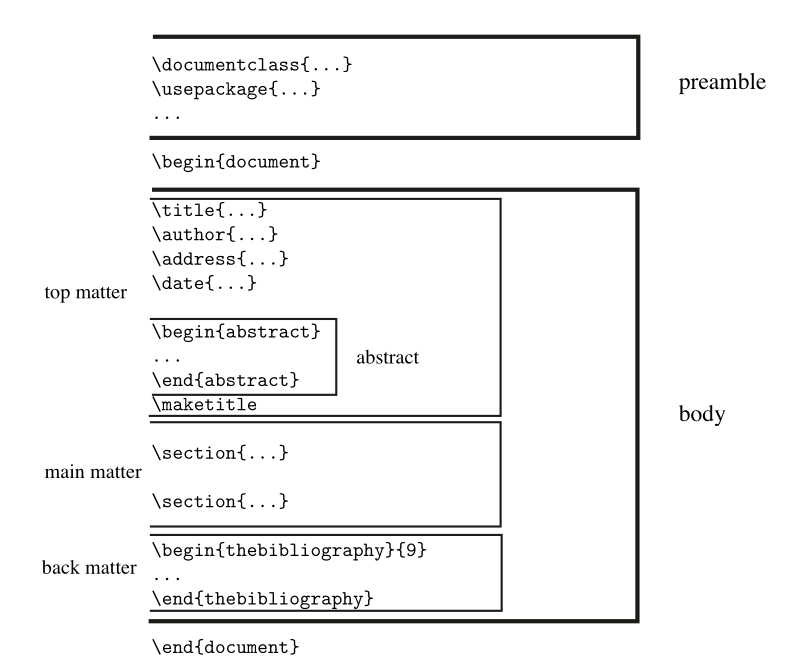
\includegraphics[width=\columnwidth]{scheme_latex_doc.png}
      }
      \onslide<3>{
          \column{0.5\textwidth}
            \begin{itemize}
              \item \textbf{preamble}: Configuración general del documento.
              \item \textbf{top matter}: Título, dedicatoria, índices, prefacio, agradecimientos, etc.
              \item \textbf{main matter}: Contenido principal del documento.
              \item \textbf{back matter}: Apéndices, bibliografía, glosario, etc.
            \end{itemize}
        \end{columns}
      }
    \end{frame} 
  \section{Paquetes}
    \subsection{Formato}
      \begin{frame}[fragile]
        \frametitle{Paquetes de formato}
        \onslide<1,2,3>{
          \justifying
          Existen diversos paquetes de formato que aumentas las posibilidades de nuestros documentos. Tenemos desde paquetes que controlan los márgenes, tamaño de papel, \emph{codificación} de caracteres, idioma, etc.

        }
        \onslide<2,3>{
          Los paquetes que veremos en esta sección serán:
          \begin{itemize}
            \item \textbf{geometry}: Configuración del documento
            \item \textbf{babel}: Idiomas
            \item \textbf{inputenc}: Codificación de caracteres.
          \end{itemize}
        }
        \onslide<3>{
          \begin{alertblock}{¿Son los únicos paquetes?}
           Pueden haber otros paquetes que hacen lo mismo, igualmente, algunas configuraciones pueden venir precargadas por defecto en algunos editores.
          \end{alertblock}
        }
      \end{frame}
      \begin{frame}[fragile]
        \frametitle{Paquete \textbf{geometry}}
        \onslide<1,2,3>{
          Podemos editar algunas opciones de márgenes o tamaño de página desde el comando \mintinline{latex}{\documentclass}, sin embargo existen mejores opciones como el paquete \href{https://ctan.org/pkg/geometry}{geometry}.

          El paquete \emph{geometry} provee una manera sencilla de controlar la geometría de la página, orientación, alineación, etc. 

        }
        \onslide<2,3>{
          \begin{block}{¿Cómo usar un paquete?}
          Todos los paquetes se importan al documento usando el \textbf{comando} \mintinline{latex}{\usepackage{geometry}}
          \end{block}

        }
        \onslide<3>{
          Algunas opciones útiles de este paquete son:
          \begin{itemize}
            \item Tamaño de papel: \textsc{letterpaper}, \textsc{a4paper}, \textsc{executivepaper}, etc
            \item Orientación: \textsc{landscape} o \textsc{portrait}
            \item Márgenes: \textsc{margin}, \textsc{left}, \textsc{right}, \textsc{top}, \textsc{bottom}.
          \end{itemize}
        }
      \end{frame}
      \begin{frame}[fragile]
        \frametitle{Otra forma de poner opciones}
        Algunos paquetes tienen comandos especiales para de definir sus opciones. Cabe remarcar que esto depende de los paquetes y no siempre es válido.
        
        \begin{listing}[H]
          \begin{minted}{latex}
            \documentclass{article}
            \usepackage{geometry}
            \usepackage[utf8]{inputenc}
            \geometry{letterpaper, top=2cm, left=2cm}
          \end{minted}
          \caption{latex3.tex}
        \end{listing} 
      \end{frame} 
      \begin{frame}[fragile]
        \frametitle{Paquete \textbf{babel}}
        \justifying
          El idioma por defecto de los documentos en \LaTeX\ es el inglés. Por lo cual escribir documentos en otros idiomas supone un esfuerzo adicional; sin embargo, hay paquetes que nos facilitan esta tarea. El paquete más usado para esta tarea es el paquete \textbf{babel} el cual se encarga de manejar las reglas tipográficas determinadas por cada lenguaje.

          Para usar el paquete \textbf{babel} basta con usar el comando \mintinline{latex}{\usepackage[option]{babel}} donde la opción será sustituida por el idioma que requiramos.

        \begin{listing}[H] 
        \begin{minted}{latex}
\documentclass{article}
\usepackage[spanish]{babel}
\begin{document}
Hola Mundo
\end{document}
        \end{minted}
          \caption{latex3.tex}
        \end{listing}
      \end{frame}
  \subsection{Escritura matemática}
    \begin{frame}[fragile]
      \frametitle{Paquetes de escritura matemática}
      \justifying
      Una de las cosas por las cuales queremos usar \LaTeX\ en ciencia es su practicidad al momento de escribir ecuaciones matemáticas. Lamentablemente, \LaTeX\ por sí solo no cuenta con todas las herramientas necesarias para escribir muchos de los símbolos matemáticos usados usualmente. Para esto necesitamos usar cualquiera de los paquetes \textbf{amsmath} o \textbf{mathtools}\footnote{Este también carga el paquete \textbf{amsmath}}.
        \begin{minted}{latex}
          \usepackage{amsmath}
          \usepackage{amsfonts}
        \end{minted}
    Existen dos formar de escribir fórmulas matemáticas en \LaTeX: el modo \emph{inline} y el modo \emph{display}. El primero servirá para escribir ecuaciones entre el texto mientras que el segundo será útil cuando se necesite un bloque de ecuaciones fuera del texto.
    \end{frame}

    \begin{frame}[fragile]
      \frametitle{Modo Inline}
      \justifying
      El modo \emph{inline} se utiliza para escribir una ecuación entre el texto, la ecuación debe de estar entre los símbolos \mintinline{latex}{$...$}:

      \begin{listing}[H]
        \begin{minted}{latex}
        La ecuación $\dfrac{1}{2}x^2$ tiene un termino al cuadrado.
        \end{minted}
        \caption{Ejemplo de modo inline}
      \end{listing}

      Otros símbolos usados para llamar al modo \emph{inline} es:
      \begin{itemize}
        \item \mintinline{latex}{\(...\)}
        \item \mintinline{latex}{\begin{math}...\end{math}}
      \end{itemize}
    \end{frame} 
    \begin{frame}[fragile]
      \frametitle{Modo Display}
      \justifying
      El modo \emph{display} sirve para poner una ecuación en un bloque separado. Se puede definir una ecuación con:

      \begin{itemize}
        \item $\mathbf{\rightarrow}$\mintinline{latex}{\[...\]}
        \item \mintinline{latex}{$$...$$}
        \item \mintinline{latex}{\begin{displaymath}...\end{displaymath}}
        \item $\mathbf{\rightarrow}$\mintinline{latex}{\begin{equation}...\end{equation}}
      \end{itemize}

      \begin{block}{Ecuaciones numeradas}
        \justifying
        En general, todos estos comandos harán que las ecuaciones sean numeradas. Sin embargo, algunas veces requerimos que las ecuaciones no sean numeradas, esto lo veremos más adelante.
      \end{block}
    \end{frame}
  \section{Cosas extras}
    \begin{frame}
      \frametitle{Cosas extras de \LaTeX}
      \justifying
      Hasta ahora hemos visto como hacer una configuración básica de un documento creado con \LaTeX. También hemos visto como escribir ecuaciones, pero hemos omitido cosas básicas que podemos hacer en los procesadores de texto usuales:

      Entre algunas cosas que \emph{básicas} se encuentran:

      \begin{itemize}
        \item Listas numeradas y no numeradas 
        \item Tablas
        \item Edición avanzada de ecuaciones matemáticas
        \item ``Objetos'' numerados y no numerados.
        \item Referencias 
      \end{itemize}
     
      Antes de avanzar hacia la última parte de este \emph{Crash course} de \LaTeX, veremos estos temas.
    \end{frame}
    \begin{frame}[fragile]
      \frametitle{Listas}
      \justifying
      Existen dos tipos de lista en \LaTeX: las listas no numeradas y las listas numeradas. Básicamente, son lo mismo, solo cambia el comando a usar. En una lista no numerada usaremos el comando \textbf{itemize} para definir su entorno:
      \begin{listing}[H]
        \begin{minted}{latex}
        \begin{itemize}
          \item Primer elemento 
          \item Segundo elemento 
          \item Tercer elemento
        \end{itemize}
        \end{minted}
        \caption{Ejemplo de lista no numerada}
      \end{listing}

      Algo importante a remarcar es que podemos hacer listas dentro de listas.
    \end{frame}
    \begin{frame}[fragile]
      \frametitle{Listas numeradas}
      \justifying
      Para hacer una lista numerada necesitamos el \emph{entorno} \textbf{enumerate}:
      \begin{listing}[H]
        \begin{minted}{latex}
        \begin{enumerate}
          \item Primer elemento 
          \item Segundo elemento 
          \item Tercer elemento
        \end{enumerate}
        \end{minted}
        \caption{Ejemplo de lista numerada}
      \end{listing}

      También se pueden hacer listas dentro de listas.
    \end{frame}
    \begin{frame}[fragile]
      \frametitle{Tablas en \LaTeX}
      \justifying
      La creación de tablas en \LaTeX\ es ``sencilla''. El entorno a usar será \textbf{tabular}:
      \begin{listing}[H]
        \begin{minted}{latex}
        \begin{tabular}{c c c}
          a & b & c \\
          d & e & f \\
          g & h & i
        \end{tabular}
        \end{minted}
        \caption{Ejemplo de una tabla}
      \end{listing}
    \end{frame}
    \begin{frame}[fragile]
      \frametitle{Tablas en \LaTeX\ (Ejemplo Terminado)}
      \justifying
      \begin{listing}[H]
        \begin{minted}{latex}
        \begin{table}
          \begin{center}
            \begin{tabular}{|c|c|c|}
              \hline
              A & B & C\\
              \hline
              a & b & c \\
              d & e & f \\
              g & h & i \\
              \hline
            \end{tabular}
          \end{center}
          \caption{Tabla de ejemplo}
        \end{table}
        \end{minted}
        \caption{Ejemplo de una tabla}
      \end{listing}
    \end{frame}
    \begin{frame}[fragile]
      \frametitle{Ecuaciones matemáticas II}
      \justifying
      Cuando escribimos ecuaciones matemáticas pueden darse diversas situaciones, por ejemplo, que haya ecuaciones multilínea
      \begin{listing}[H]
        \begin{minted}{latex}
        \begin{equation}
        \begin{split}
        A & = \frac{\pi r^2}{2} \\
         & = \frac{1}{2} \pi r^2
        \end{split}
        \end{equation} 
        \end{minted}
        \caption{Ejemplo de ecuaciones multilínea}
      \end{listing}
    \end{frame}
    \begin{frame}[fragile]
      \frametitle{Ecuaciones matemáticas II}
      \justifying
      \begin{listing}[H]
        \begin{minted}{latex}
        \begin{multline*}
        p(x) = 3x^6 + 14x^5y + 590x^4y^2 + 19x^3y^3\\ 
        - 12x^2y^4 - 12xy^5 + 2y^6 - a^3b^3
        \end{multline*}

        \begin{align*} 
        2x - 5y &=  8 \\ 
        3x + 9y &=  -12
        \end{align*}
        \end{minted}
        \caption{Ejemplo de ecuaciones multilínea}
      \end{listing}
    \end{frame}

    \begin{frame}[fragile]
      \frametitle{Ecuaciones matemáticas II}
      \justifying
      \begin{listing}[H]
        \begin{minted}{latex}
        \begin{align*}
        x&=y           &  w &=z              &  a&=b+c\\
        2x&=-y         &  3w&=\frac{1}{2}z   &  a&=b\\
        -4 + 5x&=2+y   &  w+2&=-1+w          &  ab&=cb
        \end{align*}

        \begin{gather*} 
        2x - 5y =  8 \\ 
        3x^2 + 9y =  3a + c
        \end{gather*}
        \end{minted}
        \caption{Ejemplo de ecuaciones multilínea}
      \end{listing}
    \end{frame}
    \begin{frame}[fragile]
      \frametitle{Numeración o no}
      \justifying
      Tenemos ciertos elementos que son enumerados en \LaTeX\ como las ecuaciones, capítulos, tablas, etc. Dependiendo de la situación podríamos encontrar que no necesitamos la numeración automática. Existe una convención de algunos comando que solo es necesario poner una $\star$ después del nombre del comando para quitar esa numeración.

      \begin{listing}[H]
        \begin{minted}{latex}
          \section*{Sección de prueba}
          \subsection*{Subsección de prueba}

          \begin{equation*}
            x^2 +1 = 0
          \end{equation*}
        \end{minted}
        \caption{Ejemplo de algunos comandos sin numeración}
      \end{listing}
    \end{frame}
    \begin{frame}[fragile]
      \frametitle{Referencias a otros objetos de \LaTeX}
      \LaTeX\ tiene un sistema de numeración automático para la mayoría de elementos que puede haber en un documento: capítulos, secciones, ecuaciones, tablas, figuras, etc.

      Además de mantener un orden en el contenido presentado, estos números pueden servir para ser referenciados en el texto.

      Para poder referenciar un objeto numerado necesitamos asignarle una \textbf{etiqueta} para poder identificarlo, esto se hace con el comando \mintinline{latex}{\label{etiqueta}}. Por ejemplo si queremos asignarle una etiqueta a un objeto, podemos hacerlo de la siguiente manera:

      \begin{listing}[H]
        \begin{minted}{latex}
          \section{Sección de prueba}\label{sec_prueba}
        \end{minted}
        \caption{Asignando una etiqueta a una sección}
      \end{listing}
    \end{frame}
    \begin{frame}[fragile]
      \frametitle{Referencias a otros objetos de \LaTeX}
      Una vez que ya tenemos nuestro objeto con una etiqueta y queremos referenciarlo en otra parte del texto usamos el comando \mintinline{latex}{\ref{etiqueta}}. Por ejemplo:
      \begin{listing}[H]
        \begin{minted}{latex}
          Como se muestra la \ref{sec_prueba}
        \end{minted}
        \caption{Asignando una etiqueta a una sección}
      \end{listing}

      Esto se puede realizar con todo \textit{objeto} numerado en un documento: tablas, figuras, ecuaciones, gráficas, etc. Incluso, \LaTeX\ reasignará los números si un nuevo objeto es insertado en medio de los objetos ya existentes.
      
    \end{frame}
  \section{Paquetes varios}
  \subsection{Imágenes}
  \begin{frame}[fragile]
    \frametitle{Agregar imágenes}
    \justifying
    En \LaTeX\ es posible agregar imágenes por medio del paquete \mintinline{latex}{graphicx}.
    \begin{listing}[H]
      \begin{minted}{latex}
        \usepackage{graphicx}
        \begin{figure}
          \begin{center}
            \includegraphics[scale=1]{nombre.png}
          \end{center}
          \caption{Descripcion}\label{fig:test}
        \end{figure}
      \end{minted}
      \caption{Agregando una figura}
    \end{listing}
  {\color{red}Importante}: \LaTeX\ tratará de acomodar las imágenes, y tablas, de manera automática.

  \end{frame}
  \subsection{Colores}
  \begin{frame}[fragile]
    \frametitle{Color en \LaTeX}
    \justifying
    En \LaTeX\ es posible agregar colores con el paquete \mintinline{latex}{xcolor}.
    \begin{itemize}
      \item \mintinline{latex}{Texto \textcolor{red}{de} prueba}: Texto \textcolor{red}{de} prueba
      \item \mintinline{latex}{Texto \colorbox{orange}{de} prueba}: Texto \colorbox{orange}{de} prueba
      \item \mintinline{latex}{Texto {\color{purple}de} prueba}: Texto {\color{purple}de} prueba
      \item \mintinline{latex}{\color{green} \rule{\linewidth}{0.5mm}}
    \end{itemize}
    {\color{green} \rule{\linewidth}{0.5mm}}

    El paquete \mintinline{latex}{xcolor} tiene varias opciones, para un estudio más detallado del uso de este paquete se recomienda ver el \href{https://ctan.org/pkg/xcolor}{manual de xcolor} o ver el \href{https://www.overleaf.com/learn/latex/Using_colors_in_LaTeX}{tutorial de xcolor de overleaf}. 
  \end{frame}
  \subsection{Bibliografía en LaTeX} 
  \begin{frame}[fragile]
    \frametitle{Manejo de bibliografía en \LaTeX}
    \justifying
    \begin{alertblock}{Paquetes de \textit{bibliografía}}
      \justifying
      Podemos encontrar al menos tres ``paquetes'' para el manejo de bibliografía: \textbf{bibtex}, \textbf{biblatex} y \textbf{natbib}. Realmente, \textbf{bibtex} es un programa de procesamiento (como \textbf{biber}), mientras que \textcolor{blue}{\textbf{biblatex}} y \textcolor{red}{\textbf{natbib}} si son paquetes de \LaTeX.

      A pesar de que tanto como \textbf{biblatex} como \textbf{natbib} son ampliamente usados, el segundo técnicamente ya no se encuentra en desarrollo. Por esta razón, en este curso aprenderemos \textbf{biblatex}. Sin embargo, los paquetes comparten cosas en común lo que hace que podamos cambiar entro uno y otro.
    \end{alertblock}
    Originalmente, \textsc{Bib}\TeX fue utilizado junto con algunos paquetes, como \textsc{natbib}, para manejar las bibliografías. Lamentablemente, estos paquetes pueden tener algunas restricciones, heredadas de \textsc{Bib}\TeX, lo que puede hacer un poco complicado su uso.

    El paquete BibLaTeX ha sido diseñado para tener más opciones y que sean fácilmente configurables. Afortunadamente, muchas cosas de otros paquetes se pueden usar con este paquete.
  \end{frame}
  \begin{frame}[fragile]
    \frametitle{Paquete BibLaTeX}
    \justifying
    Los comandos básicos para usar BibLaTeX son 
    \begin{listing}[H]
      \begin{minted}{latex}
      \usepackage{biblatex}
      \addbibresource{database.bib}
      \end{minted}
      \caption{Comandos básicos para usar BibLaTeX}
    \end{listing}
    El comando \mintinline{latex}{\addbibresource{}} nos da la posibilidad de agregar nuestro archivo ``bibliográfico'' o nuestra base de datos. Estos archivos, llamado \textit{bibliography database files} y con \textbf{extensión} \emph{.bib}, es una herencia de Bib\TeX, y es donde se encuentran todos los datos que utilizará el programa bibliográfico para mostrar la bibliografía.
    
    Fiel a la filosofía de \LaTeX, este archivo solo contendrá la información mientras que Bib\TeX\ o \textbf{biber} será el que procese la información.
  \end{frame}
  \begin{frame}[fragile]
    \frametitle{Archivos \textbf{\textit{bib}}}
    \justifying
    Estos archivos se conforman de \textit{entradas} bib\TeX. Cada una de estas entradas tienen la siguiente estructura general:
    \begin{listing}[H]
      \begin{minted}{bibtex}
      @article{greenwade93,
      author  = "George D. Greenwade",
      title   = "The {C}omprehensive {T}ex {A}rchive {N}etwork ({CTAN})",
      year    = "1993",
      journal = "TUGBoat",
      volume  = "14",
      number  = "3",
      pages   = "342--351"
      }
      \end{minted}
      \caption{Ejemplo de una entrada de un archivo .bib}
    \end{listing}
  \end{frame}
  \begin{frame}[fragile]
    \frametitle{Archivos \textbf{\textit{bib}}}
    \justifying
    Cada entrada pueden ser de distintos tipos y tener distintos campos. Podemos remarcar algunos puntos importantes sobre las entradas y sus campos:

    \begin{itemize}
      \item El tipo de referencia se indica de la forma \mintinline{bibtex}{@type}. Existen muchos tipos de referencias, entre los más comunes son los \mintinline{bibtex}{@book}, \mintinline{bibtex}{@article} y \mintinline{bibtex}{@inproceedings}
      \item Se define una \textit{etiqueta} al inicio de cada entrada bibliográfica con la que se identificará a lo largo del documento.
      \item Cada campo se escribe de la manera \mintinline{bibtex}{field_name = "value",}. Hay que tener en cuenta que en los diferentes campos de las entradas, los acentos, diéresis y diferentes símbolos se tienen que poner de la manera \textit{internacional}.
    \end{itemize}
    
    Cada uno de los paquetes bibliográficos pueden tener diferentes nombres para las entradas, pero en general se respeta el impuesto por bib\TeX.
    Se puede encontrar información sobre los diferentes tipos de entrada y sus respectivos campos \href{https://en.wikibooks.org/wiki/LaTeX/Bibliography_Management#biblatex}{aquí}
  \end{frame}
  \begin{frame}[fragile]
    \frametitle{Mostrando la bibliografía y citando fuentes}
    Todos los elementos que necesitemos citar deben de estar presentes en nuestro archivo \textit{bib}. Hay tres comandos especiales para citar:
    \begin{itemize}
      \item \mintinline{latex}{\cite}: El más básico de los tres, que imprime la cita sin ningún tipo de paréntesis (exceptuando cuando se pone el estilo numeric).
      \item \mintinline{latex}{\parencite}: Imprime la cita con paréntesis (exceptuando cuando se usa el modo alphabetic o numeric).
      \item \mintinline{latex}{\footcite}: Pone la cita en una nota al pie de página.
    \end{itemize}
    
    Cualquiera de los tres comandos anteriores citará las fuentes si se encuentran en el archivo \textit{bib}. Pero esto no hará que imprima bibliografía. Para esto habrá que usar el comando \mintinline{latex}{\printbibliography}.
  \end{frame}
  \begin{frame}[fragile]
    \frametitle{Estilo de bibliografía}
    Una vez que se tiene el archivo \textit{bib}, se ha mostrado la bibliografía con el comando \mintinline{latex}{\printbibliography}, y se han citado las fuentes bibliográficas (dependiendo de la configuración, solo se mostraran las fuentes bibliográficas que se han citado), podemos ver diferentes estilos de la bibliografía.

    Existen muchos estilos ya predefinidos que pueden revisarse en la \href{https://mirror.ox.ac.uk/sites/ctan.org/macros/latex/contrib/biblatex/doc/biblatex.pdf}{documentación} del biblatex, algunas de ellas son

    \begin{itemize}
      \item El estilo numeric: en la cita solo mostrará el número de la fuente bibliográfica.
      \item El estilo alphabetic: mostrará las siglas del trabajo entre corchetes.
      \item El estilo reading: mostrará autores y título en la cita
      \item El estilo authoryear: mostrará el autor y el año en la cita de la fuente
    \end{itemize}

    Estos estilos solo son un ejemplo, hay muchos estilos que pueden usarse. Igualmente, son muchas las opciones con las cuales podemos modificar como se muestran las fuentes bibliográficas lo cual hace prácticamente imposible que podamos ver cada una de ellas en este curso corto de \LaTeX.
    
  \end{frame}
  \begin{frame}[fragile]
    \frametitle{Conclusiones}
    \LaTeX\ es una poderosa herramienta de creación de documentos.
    \begin{columns}
      \begin{column}{0.5\textwidth}
        \justifying
        \begin{itemize}
          \item \LaTeX\ es extremadamente poderoso al separar el contenido y el formato.
          \item El uso de paquetes hace que las posibilidades en la creación de documentos sea muy grande.
          \item Los paquetes hacen que tenga herramientas de otros editores de texto, pero con un uso más sencillo.
          \item Tiene una curva de aprendizaje mucho más grande que otros editores de texto, pero a largo plazo es una mejor herramienta.
        \end{itemize} 
      \end{column}
      \begin{column}{0.5\textwidth}
        \begin{figure}
          \begin{center}
            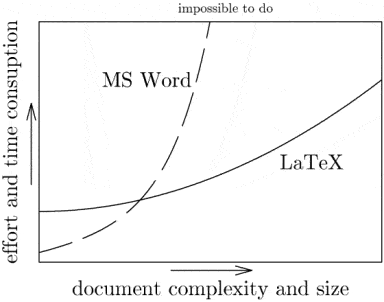
\includegraphics[width=0.95\textwidth]{figures/latex_lc.png}
          \end{center}
          \caption{}\label{fig:}
        \end{figure}
           
      \end{column}
    \end{columns}
  
  \end{frame}
\end{document}

